% --
% appendix

%\addcontentsline{toc}{chapter}{Appendix}
\addpart*{Appendix}


% --
% appendix additionals

\chapter{Appendix: Notations}
% --
% ipa

\section{International Phonetic Alphabet}\label{sec:appendix_ipa}
The International Phonetic Alphabet (IPA) are symbols that describe the pronouncing of phonemes.
A word formed with letters from a natural language alphabet does not necessarily represent the pronunciation of that word.
Therefore, many dictionaries provide an IPA transcription in order to avoid misconceptions in pronunciation.
The plots in some sections within this thesis contain transcriptions with IPA characters.
Some of the more special ones are described in \rtab{appendix_ipa}.

% ipa table
\begin{table}[ht!]
\small
\begin{center}
\caption{IPA symbols and the silence symbol with phonetic descriptions.}
\begin{tabular}{ M{2cm}  M{11cm} }
\toprule
\textbf{IPA Symbol} & \textbf{Meaning} \\
\midrule
\textturnv & back vowel: \enquote{A}, open-mid roundend mouth \\
\textupsilon & back vowel: between \enquote{O} and \enquote{U}, nearly closed rounded mouth\\
\textinvglotstop & glottal stop\\
\midrule
sil & silence, no ipa symbol!\\
\bottomrule
\label{tab:appendix_ipa}
\end{tabular}
\end{center}
\vspace{-4mm}
\end{table}
\FloatBarrier
\noindent



% --
% mathematical notations

\section{Mathematical Notations}\label{sec:appendix_math}
Vectors and scalars are usually written in small letters with vectors marked as bold symbols.
In general mathematical convention, the vectors are assumed to be column vectors.
Capital Letters are often representing matrices or fixed integer numbers, for instance, the length of a signal window $N$.
The dimension of vectors and matrices, such as $\bm{x} \in \R^n$ or $X \in \C^{M \times N}$, are usually provided and placed next to their formulation, otherwise they follows from the context.
Some symbols like $n$ or $x$ are likewise used in different sections but with different meaning and representation and should hopefully not confuse the reader of this thesis.
The logarithm notation $\log x$ without subscription is always referred to the natural logarithm of basis $e$.


% --
% appendix experiments

\chapter{Appendix: Experiments}

\section{Dataset}

\subsection{Not Randomizing Onsets}
The extraction of a time interval of \SI{500}{\milli\second} from the original recordings required the use of an accurate onset detection.
The onsets were determined as described in \rsec{signal_onset}, however, it appeared to be advantageous to randomize the onset positions by a few frames to generalize better upon shift invariance.
To evaluate the difference to the experiments in \rsec{exp} that use randomized onsets, a separate experiment was performed without randomizing the onset positions.
\rtab{exp_fs_rand_frames_l12} shows the results of not randomizing the frame onsets, which can be directly compared with the results in \rtab{exp_fs_cepstral_l12}.
\begin{table}[ht!]
\small
\begin{center}
\caption{Experiment of not randomizing frame positions, trained on different networks with 12 cepstral coefficients, no frame-based normalization and 1000 epochs.}
\begin{tabular}{ M{3cm}  M{2cm}  M{2cm}  M{2.5cm}  M{2.5cm} }
\toprule
\textbf{arch} & \textbf{mfcc} & \textbf{norm} & \textbf{acc test} & \textbf{acc my} \\
\midrule
conv-trad & 12 & 0 & $82.13 \pm 0.74$ & $84.00 \pm 5.66$ \\
conv-fstride &12 & 0 & $73.60 \pm 1.59$ & $66.40 \pm 5.43$ \\
conv-jim & 12 & 0 & $78.07 \pm 0.77$ & $73.60 \pm 7.42$ \\
\bottomrule
\label{tab:exp_fs_rand_frames_l12}
\end{tabular}
\end{center}
\vspace{-4mm}
\end{table}
\FloatBarrier
\noindent
By not randomizing the onsets the results of the \texttt{conv-trad} and the \texttt{conv-fstride} model improved slightly, while the performance of the \texttt{conv-jim} was not much affected, probably because of the striding in the frame dimension.

\subsection{Labels and Dataset Splits}
The available labels and the datasets splits of the speech commands dataset \cite{Warden2018} used for training, validation, and testing are listed in \rtab{exp_dataset_all_labels}.
\begin{table}[ht!]
\small
\begin{center}
\caption{All labels and counts of available data examples for each set, obtained from the speech commands dataset \texttt{v0.02}.}
\begin{tabular}{ M{2cm}  M{1.75cm}  M{1.75cm}  M{1.75cm}  M{1.75cm} }
\toprule
\textbf{label} & \textbf{train} & \textbf{test} & \textbf{validation} & \textbf{total} \\
\midrule
backward & 1346 & 165 & 153 & 1664 \\
bed & 1624 & 234 & 213 & 2071 \\
bird & 1697 & 185 & 182 & 2064 \\
cat & 1657 & 194 & 180 & 2031 \\
dog & 1711 & 220 & 197 & 2128 \\
down & 3134 & 406 & 377 & 3917 \\
eight & 3033 & 408 & 346 & 3787 \\
five & 3240 & 445 & 367 & 4052 \\
follow & 1275 & 172 & 132 & 1579 \\
forward & 1256 & 155 & 146 & 1557 \\
four & 2955 & 400 & 373 & 3728 \\
go & 3106 & 402 & 372 & 3880 \\
happy & 1632 & 203 & 219 & 2054 \\
house & 1727 & 191 & 195 & 2113 \\
learn & 1286 & 161 & 128 & 1575 \\
left & 3037 & 412 & 352 & 3801 \\
marvin & 1710 & 195 & 195 & 2100 \\
nine & 3170 & 408 & 356 & 3934 \\
no & 3130 & 405 & 406 & 3941 \\
off & 2970 & 402 & 373 & 3745 \\
on & 3086 & 396 & 363 & 3845 \\
one & 3140 & 399 & 351 & 3890 \\
right & 3019 & 396 & 363 & 3778 \\
seven & 3205 & 406 & 387 & 3998 \\
sheila & 1606 & 212 & 204 & 2022 \\
six & 3088 & 394 & 378 & 3860 \\
stop & 3111 & 411 & 350 & 3872 \\
three & 2966 & 405 & 356 & 3727 \\
tree & 1407 & 193 & 159 & 1759 \\
two & 3111 & 424 & 345 & 3880 \\
up & 2948 & 425 & 350 & 3723 \\
visual & 1288 & 165 & 139 & 1592 \\
wow & 1724 & 206 & 193 & 2123 \\
yes & 3228 & 419 & 397 & 4044 \\
zero & 3250 & 418 & 384 & 4052 \\
\_noise\footnotemark & 2863 & 357 & 357 & 3577 \\
\bottomrule
\label{tab:exp_dataset_all_labels}
\end{tabular}
\end{center}
\vspace{-4mm}
\end{table}
\FloatBarrier
\noindent
\footnotetext{The noise label was added from the provided noise files, as described in \rsec{exp_dataset_structure}.}



% --
% weights

\section{Trained Weights from the Final Experiments}\label{sec:appendix_weights}
The trained weights from the final experiments in \rsec{exp_final} are shown in \rfig{exp_final_weights_conv-trad}, \rfig{exp_final_weights_conv-fstride} and \rfig{exp_final_weights_conv-jim} for each model separately.
\begin{figure}[!ht]
  \centering
  \subfigure[Norm.: 0]{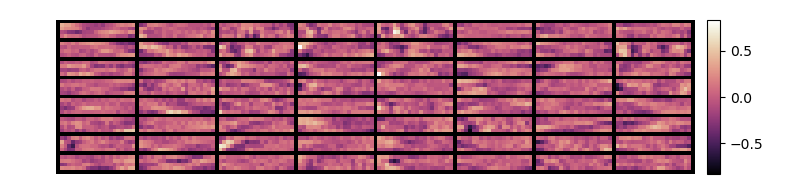
\includegraphics[width=0.48\textwidth]{./5_exp/figs/exp_final_weights_conv-trad_norm0_conv1.png}}
  \quad
  \subfigure[Norm.: 0, div. color]{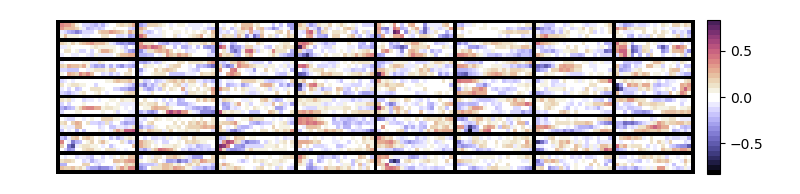
\includegraphics[width=0.48\textwidth]{./5_exp/figs/exp_final_weights_conv-trad_norm0_div_conv1.png}}
  \subfigure[Norm.: 1]{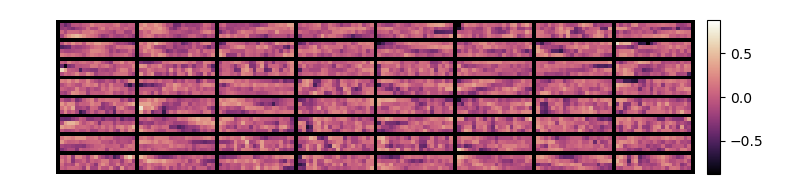
\includegraphics[width=0.48\textwidth]{./5_exp/figs/exp_final_weights_conv-trad_norm1_conv1.png}}
  \quad
  \subfigure[Norm.: 1, div. color]{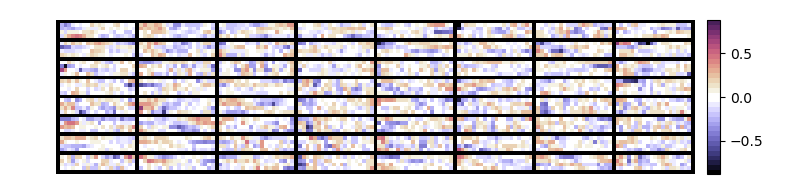
\includegraphics[width=0.48\textwidth]{./5_exp/figs/exp_final_weights_conv-trad_norm1_div_conv1.png}}
  \caption{Weights of the first convolutional layer of the \texttt{conv-trad} model from the final experiments showed in \rsec{exp_final} visualized with a continuous and diverging color scheme.}
  \label{fig:exp_final_weights_conv-trad}
\end{figure}
\FloatBarrier
\noindent

\begin{figure}[!ht]
  \centering
  \subfigure[Norm.: 0]{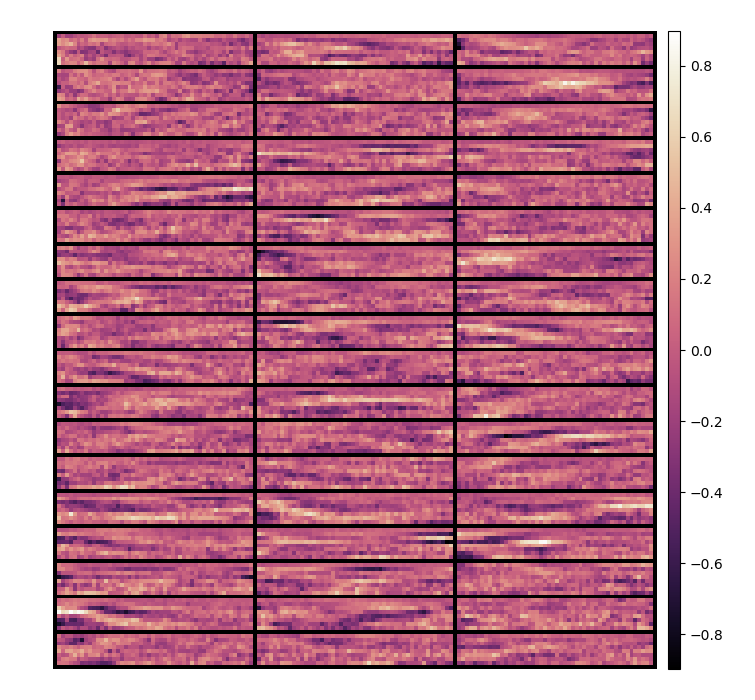
\includegraphics[width=0.48\textwidth]{./5_exp/figs/exp_final_weights_conv-fstride_norm0_conv.png}}
  \quad
  \subfigure[Norm.: 0, div. color]{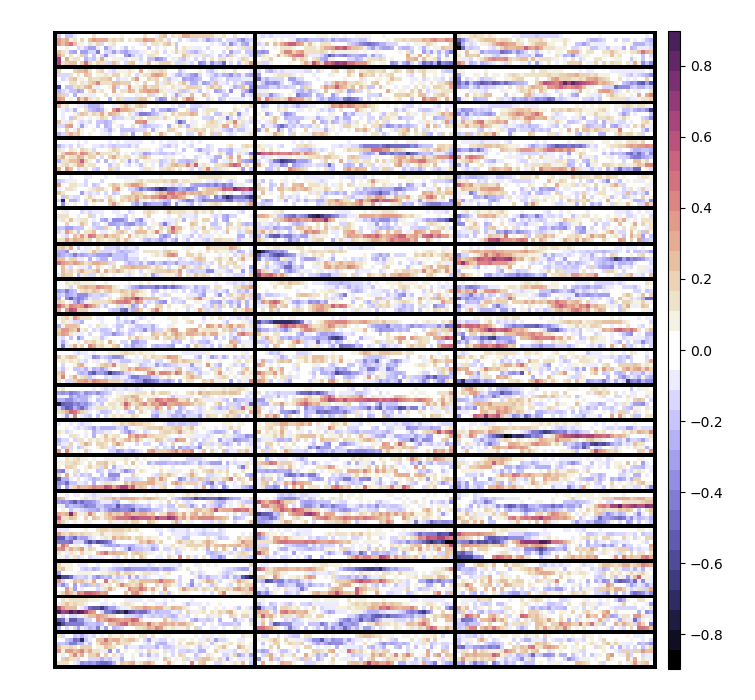
\includegraphics[width=0.48\textwidth]{./5_exp/figs/exp_final_weights_conv-fstride_norm0_div_conv.png}}
  \subfigure[Norm.: 1]{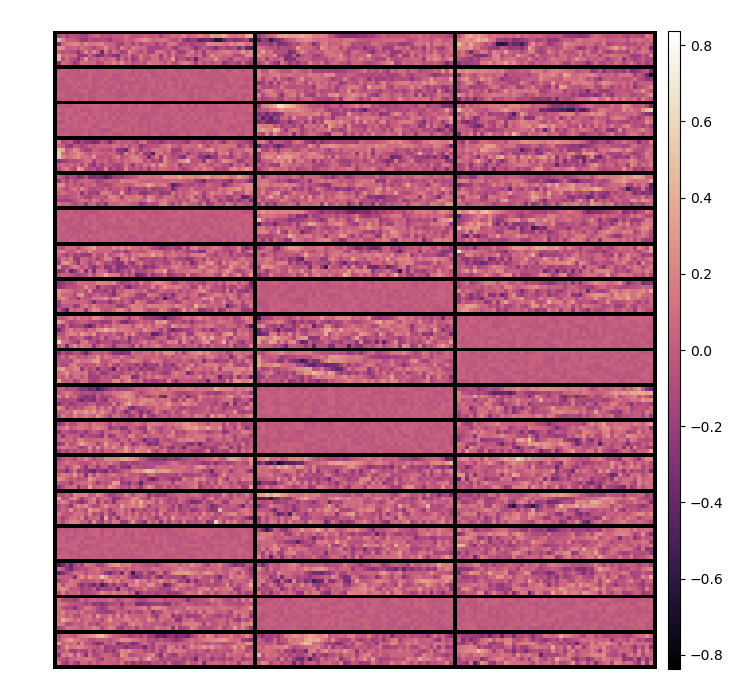
\includegraphics[width=0.48\textwidth]{./5_exp/figs/exp_final_weights_conv-fstride_norm1_conv.png}}
  \quad
  \subfigure[Norm.: 1, div. color]{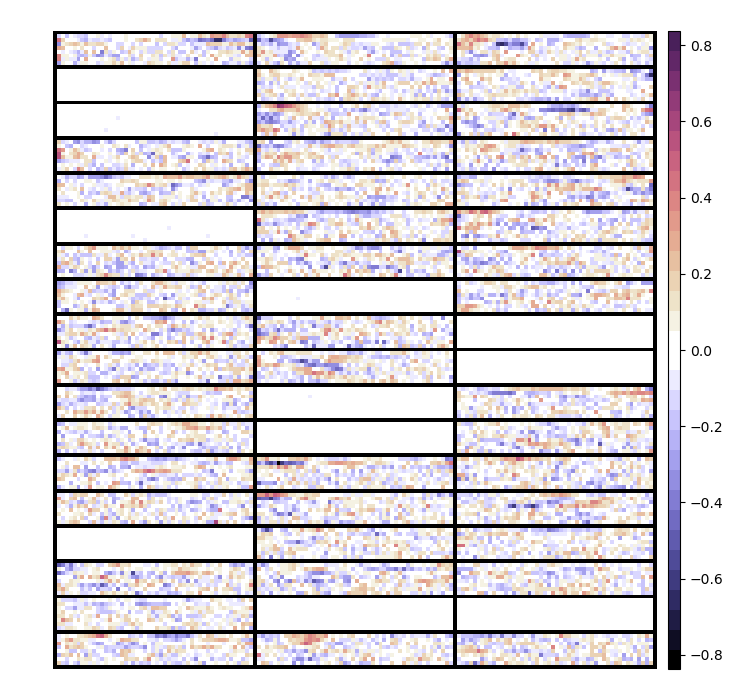
\includegraphics[width=0.48\textwidth]{./5_exp/figs/exp_final_weights_conv-fstride_norm1_div_conv.png}}
  \caption{Weights of the first convolutional layer of the \texttt{conv-fstride} model from the final experiments showed in \rsec{exp_final} visualized with a continuous and diverging color scheme.}
  \label{fig:exp_final_weights_conv-fstride}
\end{figure}
\FloatBarrier
\noindent

\begin{figure}[!ht]
  \centering
  \subfigure[Norm.: 0]{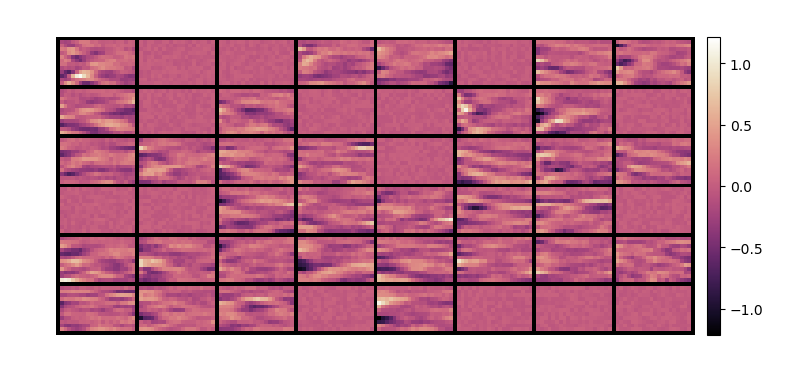
\includegraphics[width=0.48\textwidth]{./5_exp/figs/exp_final_weights_conv-jim_norm0_conv_layer0.png}}
  \quad
  \subfigure[Norm.: 0, div. color]{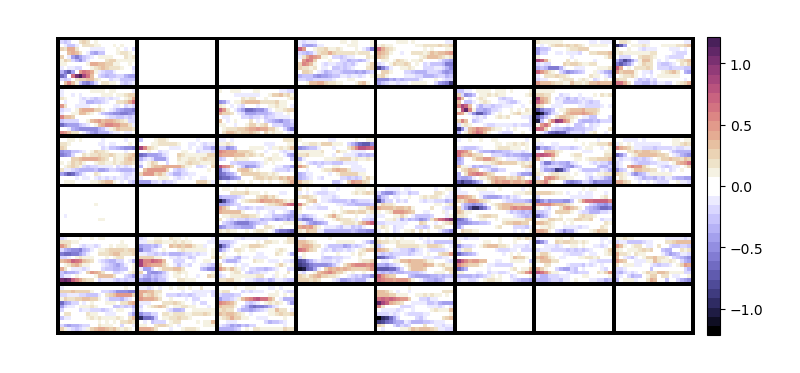
\includegraphics[width=0.48\textwidth]{./5_exp/figs/exp_final_weights_conv-jim_norm0_div_conv_layer0.png}}
  \subfigure[Norm.: 1]{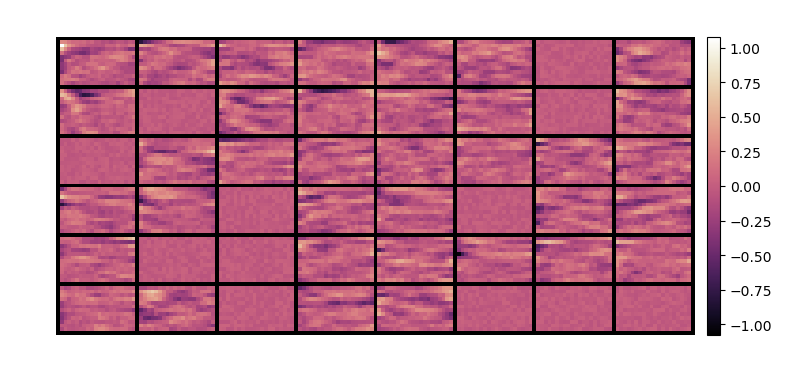
\includegraphics[width=0.48\textwidth]{./5_exp/figs/exp_final_weights_conv-jim_norm1_conv_layer0.png}}
  \quad
  \subfigure[Norm.: 1, div. color]{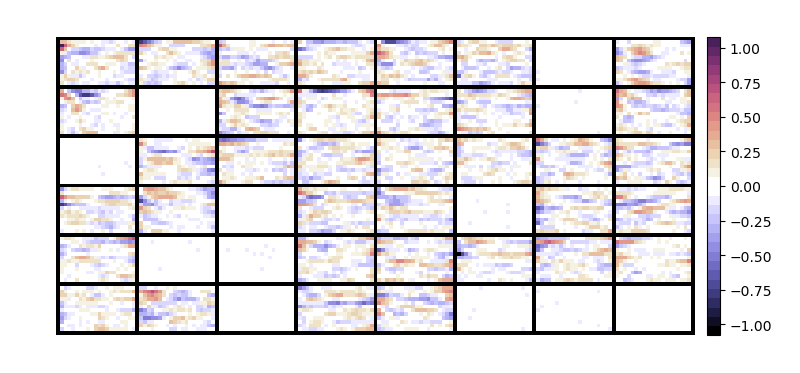
\includegraphics[width=0.48\textwidth]{./5_exp/figs/exp_final_weights_conv-jim_norm1_div_conv_layer0.png}}
  \subfigure[Norm.: 1, adv-label-g-100]{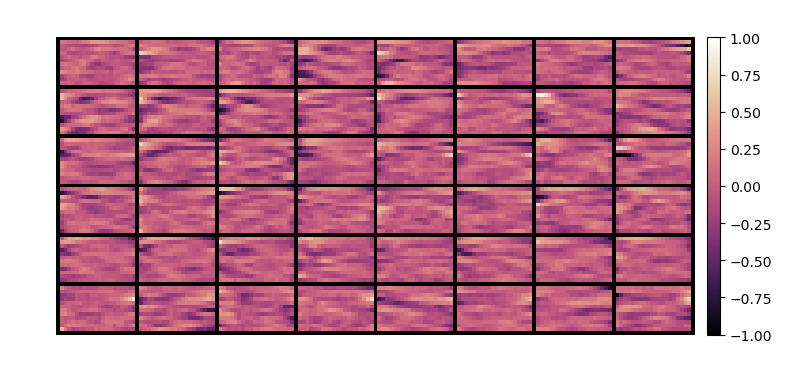
\includegraphics[width=0.48\textwidth]{./5_exp/figs/exp_final_weights_conv-jim_norm1_adv-label-g-100_conv_layer0.png}}
  \quad
  \subfigure[Norm.: 1, adv-label-g-100, div. color]{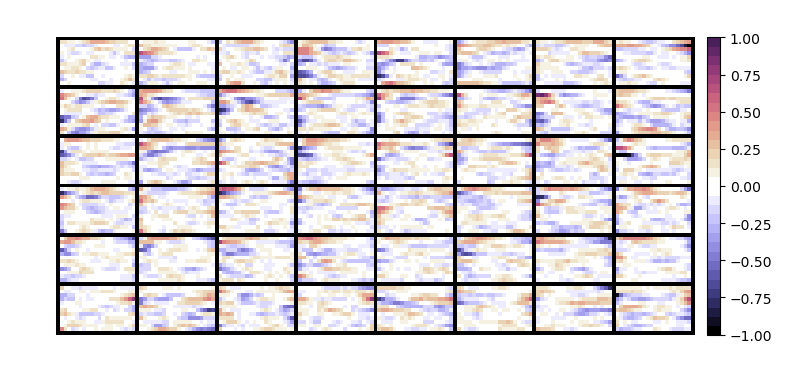
\includegraphics[width=0.48\textwidth]{./5_exp/figs/exp_final_weights_conv-jim_norm1_adv-label-g-100_div_conv_layer0.png}}
  \caption{Weights of the first convolutional layer of the \texttt{conv-jim} model from the final experiments showed in \rsec{exp_final} visualized with a continuous and diverging color scheme.}
  \label{fig:exp_final_weights_conv-jim}
\end{figure}
\FloatBarrier
\noindent